% Auto-generated by generate_slide5.py - do not edit manually
\documentclass[border=12pt]{standalone}
\usepackage{fontspec}
\setmainfont{Carlito}
\usepackage{xcolor}
\usepackage{graphicx}
\usepackage{tikz}
\usetikzlibrary{positioning,calc}

\definecolor{canvabg}{RGB}{246,244,241}
\pagecolor{canvabg}

\begin{document}
\begin{tikzpicture}[
    panel/.style={inner sep=0pt, outer sep=0pt, anchor=center},
    colhead/.style={font=\Large\bfseries, align=center, text=black!85, inner sep=2pt},
]
    %% Top row of panels - uniform width forces strict column alignment
    \node[panel] (rev) {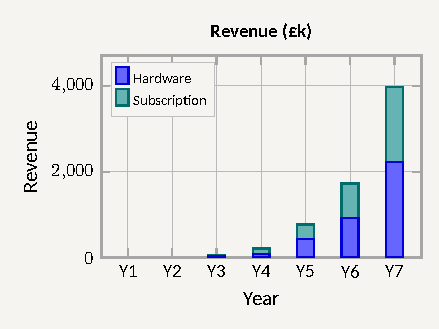
\includegraphics[width=7.0cm]{slide5_panel_revenue.pdf}};
    \node[panel, right=0.6cm of rev]  (gm)   {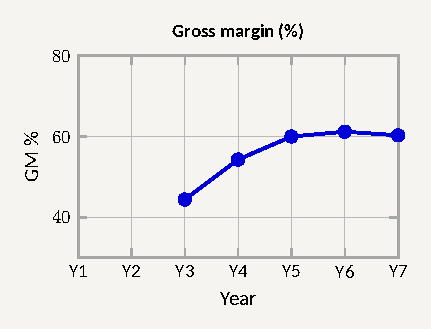
\includegraphics[width=7.0cm]{slide5_panel_gm.pdf}};
    \node[panel, right=0.6cm of gm]   (cash) {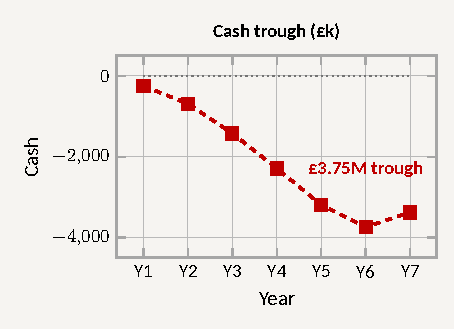
\includegraphics[width=7.0cm]{slide5_panel_cash.pdf}};

    %% Bottom row of panels - aligned vertically against top row
    \node[panel, below=0.4cm of rev]  (opex)   {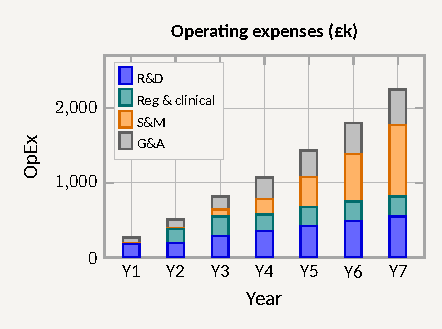
\includegraphics[width=7.0cm]{slide5_panel_opex.pdf}};
    \node[panel, below=0.4cm of gm]   (ebitda) {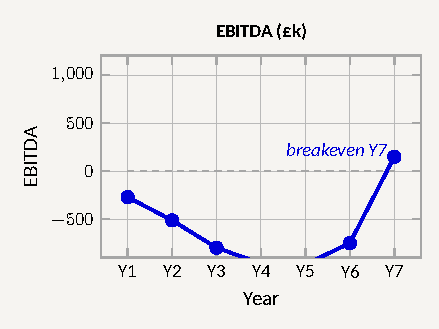
\includegraphics[width=7.0cm]{slide5_panel_ebitda.pdf}};
    \node[panel, below=0.4cm of cash] (wc)     {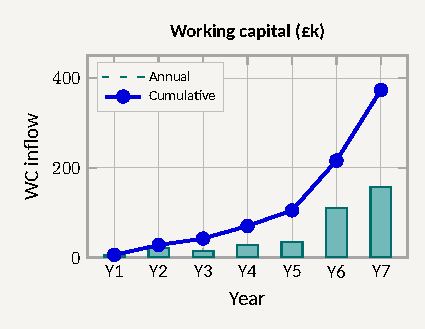
\includegraphics[width=7.0cm]{slide5_panel_wc.pdf}};

    %% Column headers - all anchored to same y line (rev.north + 14pt) so they baseline-align
    %% regardless of any panel-bbox height differences. xshift centres over the plot area.
    \node[colhead, anchor=south] at ($(rev.north)  + (12pt, 14pt)$) {Revenue and Costs};
    \node[colhead, anchor=south] at ($(rev.north -| gm)   + (12pt, 14pt)$) {Path to Profitability};
    \node[colhead, anchor=south] at ($(rev.north -| cash) + (12pt, 14pt)$) {Capital Requirement};
\end{tikzpicture}
\end{document}
